\scanpage{199}
% archive sheet number: 198

\[
 \tau=\operatorname{Tr}(x_1x_2)x_3x_4\qquad x_2x_1
\]

\figure{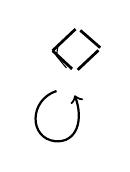
\begin{tikzpicture}[scale=.55]
\draw[line width=1pt] (0,1.4)--(.53,1.9) (.64,1.87)--(1.1,1.47) (1.06,1.41)--(.58,.96) (.45,.98)--(0,1.4);
\draw (.12,1.5)--(.09,1.28)--(.32,1);
\draw[->,line width=.8pt] (.09,.47) .. controls (-.55,.26) and (-.55,-.62) .. (.06,-.69) .. controls (.56,-.73) and (.72,-.2) .. (.51,.37);
\end{tikzpicture}}

\figure{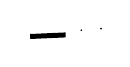
\begin{tikzpicture}\draw[line width=1.8pt] (0,0)--(.45,.02);\fill (.65,.08) circle (.012) (.9,.10) circle (.012);\end{tikzpicture}}

\[
 \tau^2-\Sigma_{(1,2),3,4}\tau+\Pi
\]

\[
 \operatorname{Tr}x_1x_2x_3\deleted{\unsure{x}}x_4+\operatorname{Tr}x_2x_1x_3x_4
\]

\[
 \begin{aligned}
 &x_1x_2x_3x_4 &x_2x_3x_4x_1&&x_3x_4x_1x_2 &x_4x_1x_2x_3\\
 &x_4x_3x_2x_1 &x_3x_2x_{\unsure{1|.}}\\
 &&&&\tau
 \end{aligned}
\]

\figure{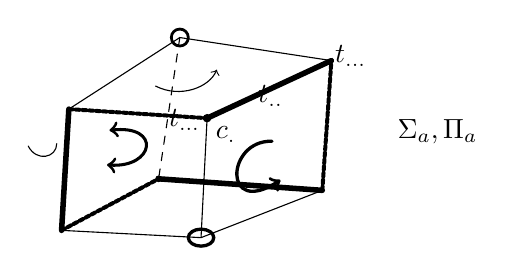
\begin{tikzpicture}[scale=.77,line cap=round]
\coordinate (a) at (0,0); \coordinate (b) at (2.3,-.12); \coordinate (c) at (4.3,.66); \coordinate (d) at (1.6,.85);
\coordinate (e) at (.12,2); \coordinate (f) at (2.4,1.85); \coordinate (g) at (4.45,2.8); \coordinate (h) at (1.95,3.18);
\draw (a)--(b)--(c)--(g)--(h)--(e)--(f)--(b);
\draw[line width=2pt] (a)--(e) (f)--(g) (d)--(c);
\draw[dashed] (h)--(d); \draw[densely dotted,line width=1.45pt] (a)--(d) (e)--(f) (c)--(g);
\draw[line width=1pt] (h) circle (.14); \draw[line width=1.2pt] (b) ellipse (.21 and .14);
\fill (f) circle (.07) (d) circle (.055);
\draw[->] (1.55,2.38) .. controls (1.96,2.17) and (2.44,2.36) .. (2.56,2.65);
\draw[<->,line width=1.1pt] (.75,1.08) .. controls (1.53,1.02) and (1.66,1.75) .. (.79,1.65);
\draw[->,line width=1.2pt] (3.47,1.47) .. controls (2.71,1.49) and (2.65,.20) .. (3.61,.83);
\draw (-.55,1.39) .. controls (-.41,1.12) and (-.08,1.2) .. (-.08,1.43);
\node at (2.03,1.82) {$t_{\ldots}$}; \node at (2.71,1.58) {$c_{.}$}; \node at (3.45,2.21) {$t_{..}$}; \node at (4.77,2.87) {$t_{\ldots}$};
\node at (6.2,1.63) {$\Sigma_a,\Pi_a$};
\end{tikzpicture}}

\[
 \deleted{\unsure{\tau^2-}}\qquad \tau^2
\]

\[
 \underline{b_s,c_s},t_s\ \big|\ \underline{t_a}\ \big|\ t_f
\]

\[
 \tau^{\unsure{\infty|8}}+\alpha_1\tau^7\mathord{\text{---}}+\alpha_8=0
\]

\uline{Nb} $\left\{\begin{aligned} b_s&=b_{s'}\\c_s&=c_{s'}\\t_a&=t_{a'}\end{aligned}\right.$

\[
 \alpha_i\in\mathbb Z[b_{..},\unsure{c_{.}},t_{..}]
\]

mais $\left\{\begin{aligned}t_s&\ne t_{s'}\\t_f&\ne t_{\unsure{f\,f'|f'}}\end{aligned}\right.$ \quad de degré $2$ sur $A^{\unsure{\mathfrak S|\mathscr S}_4}$\\ de degré $8$ sur $A^{\mathfrak S_4}$\\ \uline{de degré $6$ sur $B^{\mathfrak S_4}$}\\ de degré $8$ (?) \deleted{\unsure{?}} sur $A$

\[
 \begin{aligned}
 &g\unsure{\tau_+|x_+|\tau},\ g'\tau\quad g''\tau\\[-1pt]
 &\Sigma g\tau\\[-1pt]
 &\Sigma g
 \end{aligned}
\]

\[
 \begin{aligned}
 &\tau^\infty+\beta_1\tau^7\mathord{\text{---}}+\beta_8=0\\
 &\underbrace{(\alpha_1-\beta_1)}_{\gamma_1}\tau^7\mathord{\text{---}}+\underline{\alpha_8-\beta_8}=0
 \end{aligned}
\]

\figure{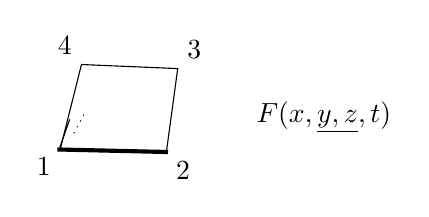
\begin{tikzpicture}[scale=.65]
\draw (.06,.12)--(.47,1.75)--(2.35,1.67)--(2.13,.05);
\draw[line width=1.5pt] (0,.09)--(2.16,.04); \draw (.05,.14)--(.24,.68); \draw[dotted] (.32,.41)--(.56,.85);
\node[above left] at (.47,1.75) {$4$};\node[above right] at (2.35,1.67) {$3$};\node[below left] at (.06,.12) {$1$};\node[below right] at (2.13,.05) {$2$};
\node[right] at (3.7,.71) {$F(x,\underline{y,z},t)$};
\end{tikzpicture}}

\[
 H\subset\mathfrak S_4
\]

\diagram{\begin{tikzcd}[ampersand replacement=\&,row sep=small]
 B^H\arrow[d,dash,"\text{degré }6"]\\ B^{\mathfrak S_4}=B^G
\end{tikzcd}}

$\alpha+\beta\tau\qquad a\quad b$ stables par $\unsure{+\mathfrak S_3^+|\mathfrak S_3^+}$

\[
 \begin{aligned}
 &\text{''}\quad\alpha'+\beta'\tau'=\alpha'+\beta'(\sigma-\tau)=(\alpha'+\beta'\sigma)-\beta'\tau\\
 &\beta'=-\beta\ /\ \alpha'\unsure{+|-}\beta\sigma=\alpha\qquad
 \alpha'=\alpha+\beta\sigma\ /\ (\alpha')'=\alpha=\alpha'+
 \end{aligned}
\]
